\documentclass{beamer}

\mode<presentation>
{
  \usetheme{Pittsburgh}
  \useoutertheme{split}
  \setbeamercovered{transparent} 
  \setbeamertemplate{navigation symbols}{}
  \setbeamertemplate{title}{}
  % \setbeamertemplate{footline}[page number]{}
  % \setbeamertemplate{footline}[frame number]
}

\usepackage{amsmath}
\usepackage[english]{babel}
\usepackage[utf8]{inputenc}
\usepackage{times}
\usepackage[T1]{fontenc}
\usepackage{graphicx}
\usepackage{hyperref}
\usepackage{subfigure}
\usepackage{setspace}
\usepackage{multirow}
\usepackage{booktabs}
\usepackage{tabulary}
\usepackage{tabu}

\title[Data Modeling and Visualisation]
{Data Modeling and Visualisation}

\author{CCT490H5F - Social Data Analytics}
\institute[] {
    Professor Alex Hanna
}

\date[] {
October 20, 2016
}

\begin{document}

\begin{frame}
  \titlepage
\end{frame}

\begin{frame}[plain]
    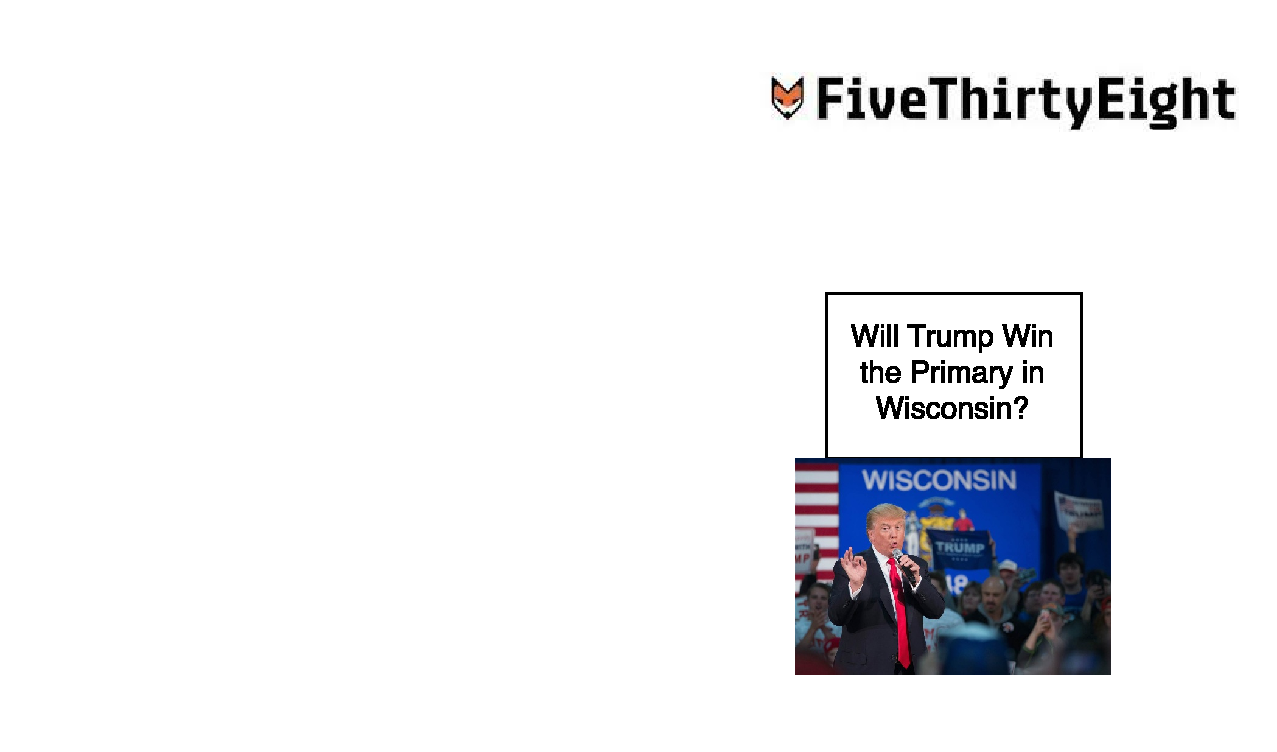
\includegraphics[width=\textwidth]{img/538-primary-1.pdf}
\end{frame}

\begin{frame}[plain]
    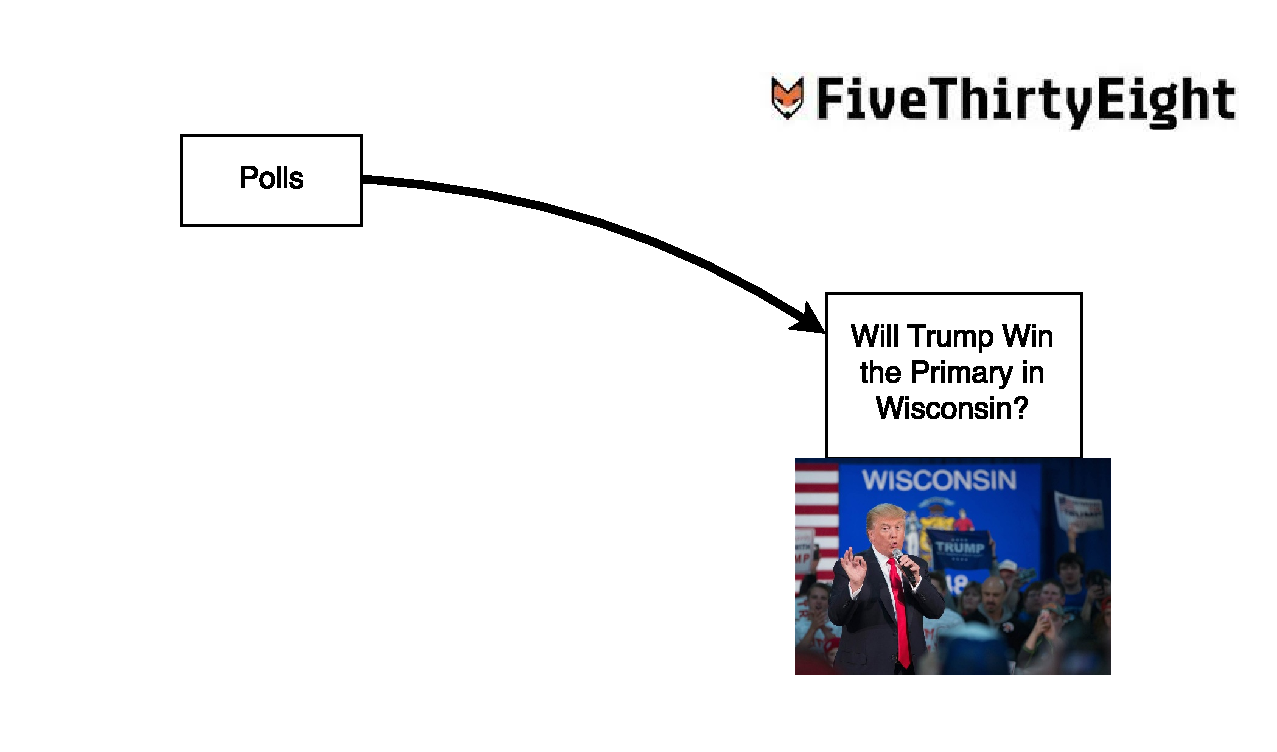
\includegraphics[width=\textwidth]{img/538-primary-2.pdf}
\end{frame}

\begin{frame}[plain]
    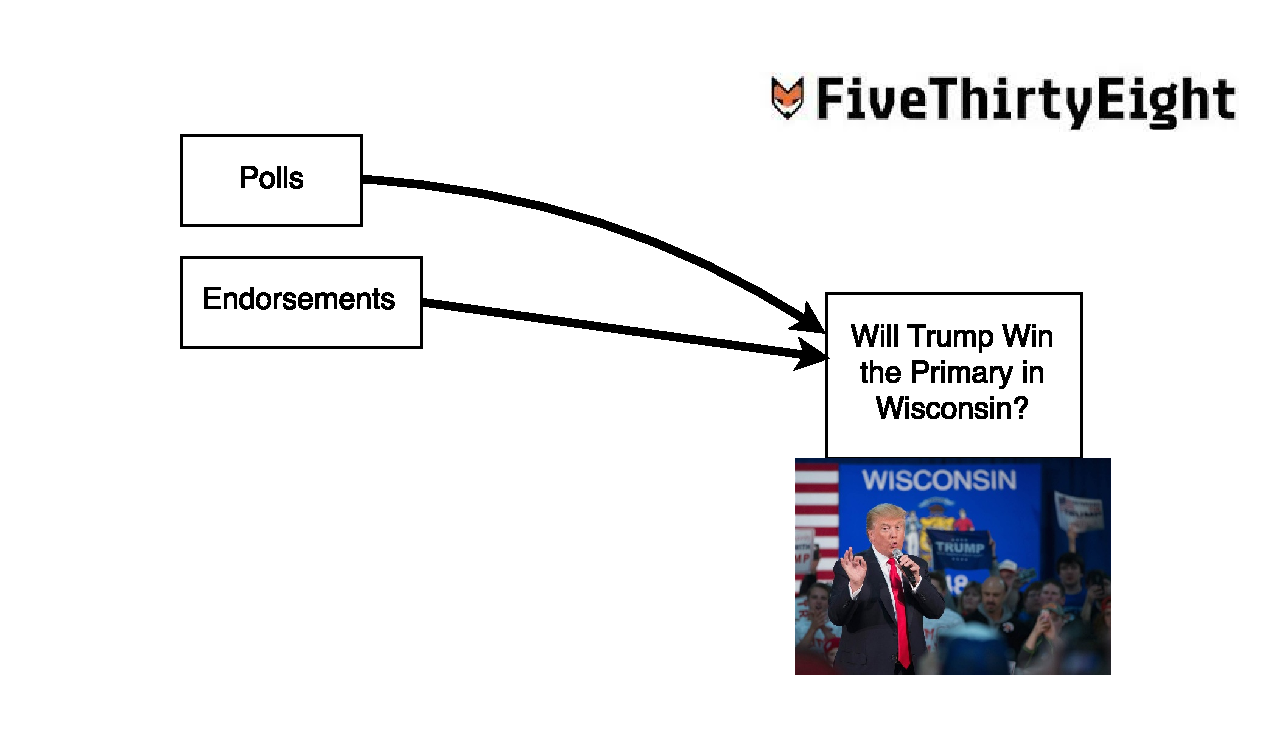
\includegraphics[width=\textwidth]{img/538-primary-3.pdf}
\end{frame}

\begin{frame}[plain]
    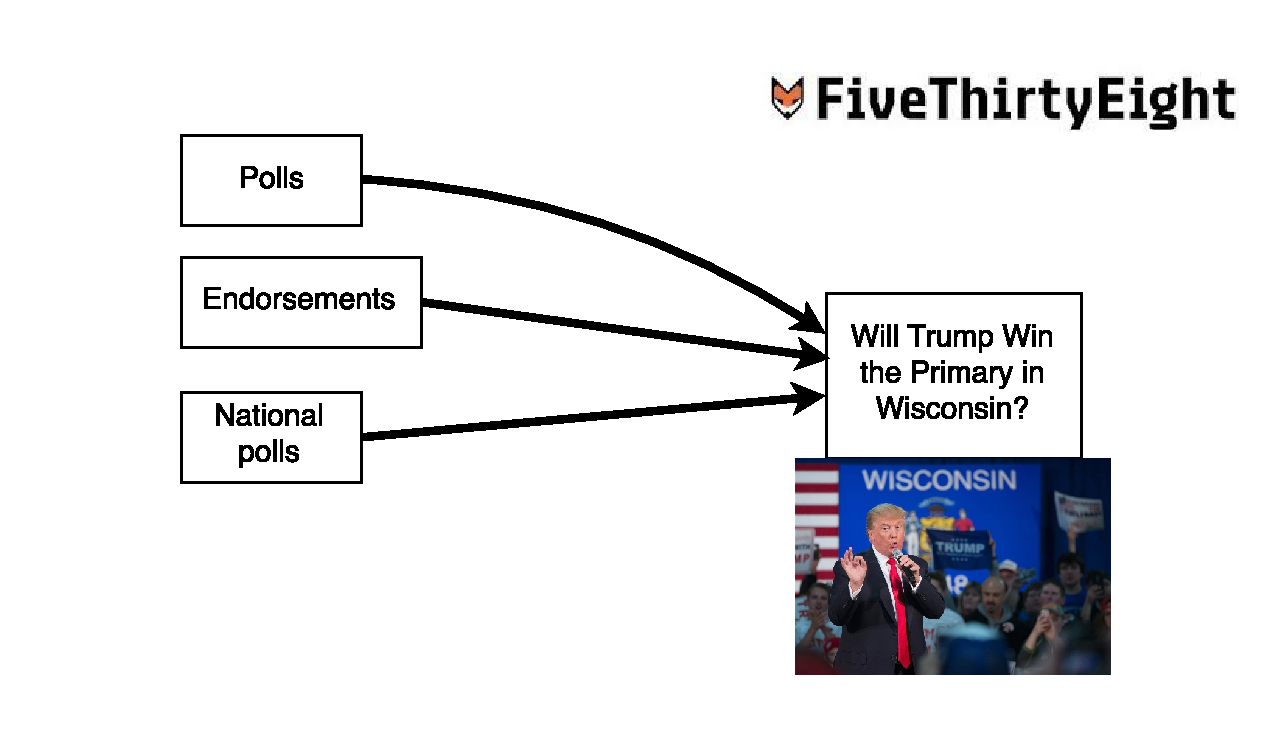
\includegraphics[width=\textwidth]{img/538-primary-4.pdf}
\end{frame}

\begin{frame}[plain]
    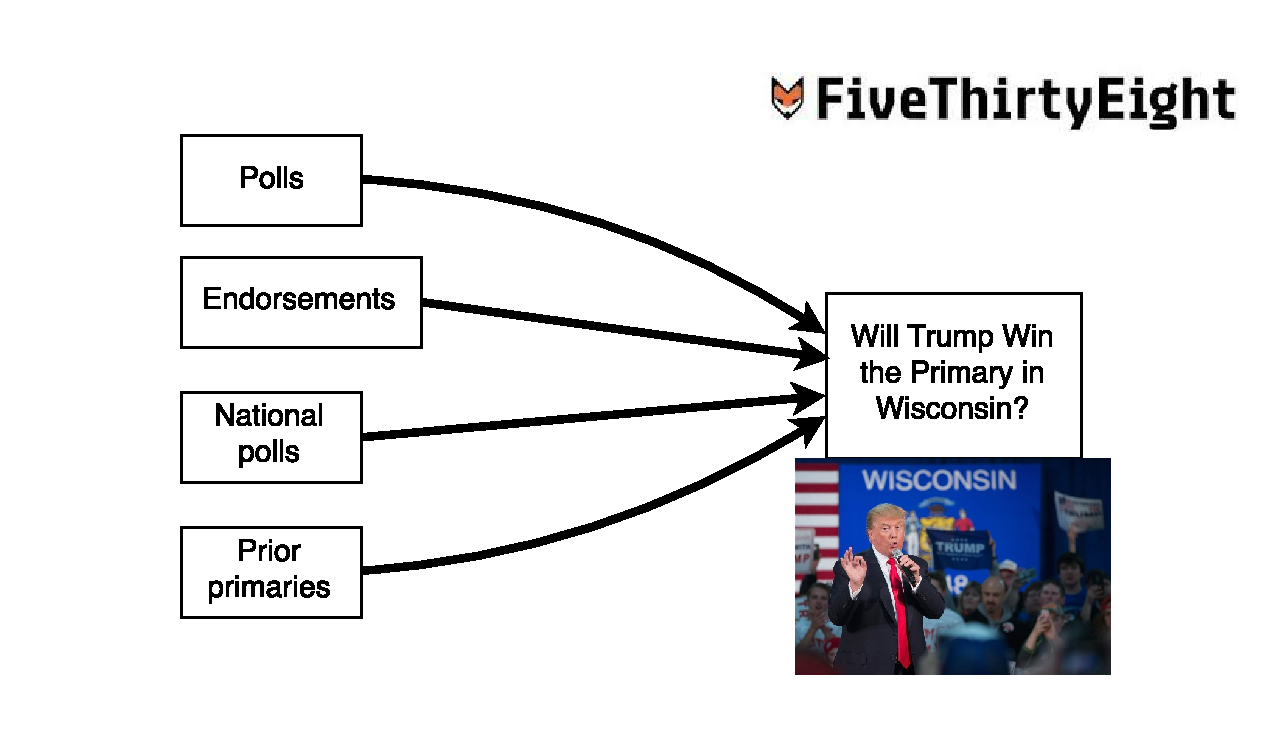
\includegraphics[width=\textwidth]{img/538-primary-5.pdf}
\end{frame}

\begin{frame}{Data Modeling}
    \begin{columns}
        \begin{column}{0.5\textwidth}
            A \textit{model} is a simplified representation of reality. \\

            \vspace*{1em}

            \only<2>{A \textit{mathematical model} is a representation of reality using numbers.}
        \end{column}
        \begin{column}{0.5\textwidth}
            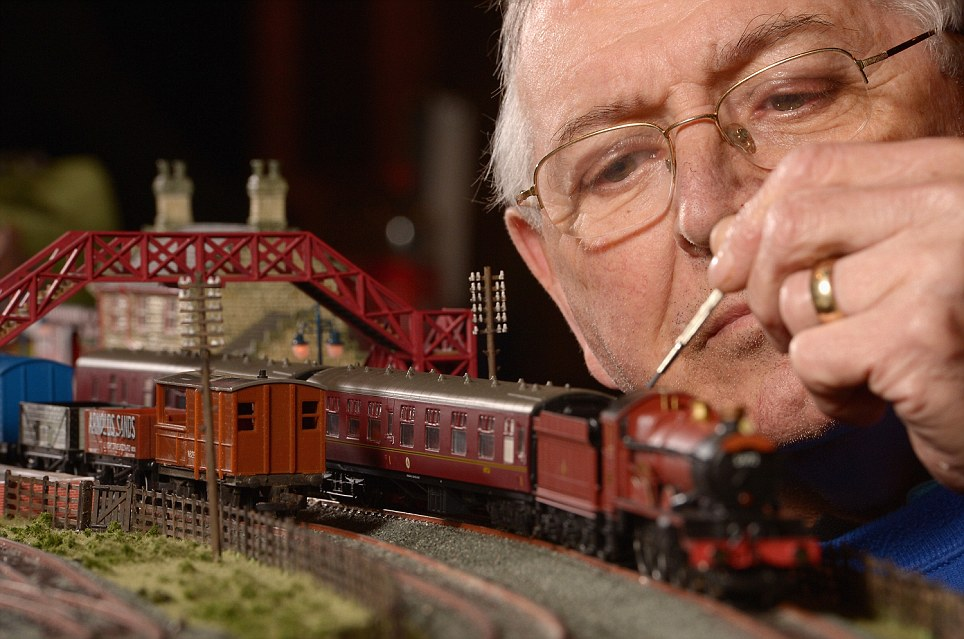
\includegraphics[width=\textwidth]{img/model-train.jpg}
        \end{column}
    \end{columns}
\end{frame}

\begin{frame}{Why have a model?}
    \begin{itemize}[<+->]
        \item \textit{Description}: You want to summarise data.
        \item \textit{Explanation}: You want replicate the working of the world with existing data.
        \item \textit{Prediction}: You want to forecast the future from past data.
    \end{itemize}
    
    \vspace*{1em}
    \visible<4->{Modeling is a \textit{data reduction} process.}

    \vspace*{1em}
    \visible<5->{``All models are wrong but some are useful.'' - George Box, statistician}
\end{frame}

\begin{frame}{Example: More Tweets, More Votes}
    \begin{columns}
        \begin{column}{0.5\textwidth}
            DiGrazia et al. 2013. ``More Tweets, More Votes: Social Media as a Quantitative Indicator of Political Behavior''

            \vspace*{1em}

            The more times a 2010 US House candidate was mentioned, the more likely it is they will be elected.
        \end{column}
        \begin{column}{0.5\textwidth}
            Other things which affect votes
            \begin{itemize}
                \item Incumbency
                \item Ideological leaning
                \item Age
                \item Education
                \item Gender
                \item Race
                \item Media markets
            \end{itemize}
        \end{column}
    \end{columns}
\end{frame}

\begin{frame}{Major variables in MTMV}
    Critical variables for this analysis
    \begin{itemize}[<+->]
        \item \textit{Dependent variable}: Republican percent of the vote share (\texttt{vote\_share})
        \item \textit{Independent variables}
        \begin{itemize}
            \item Republican percent of Twitter mention share (\texttt{mshare})
            \item Republican incumbency (\texttt{rep\_inc})
        \end{itemize}
    \end{itemize}
\end{frame}

\begin{frame}{Description of MTMV Data: Crosstabs}
    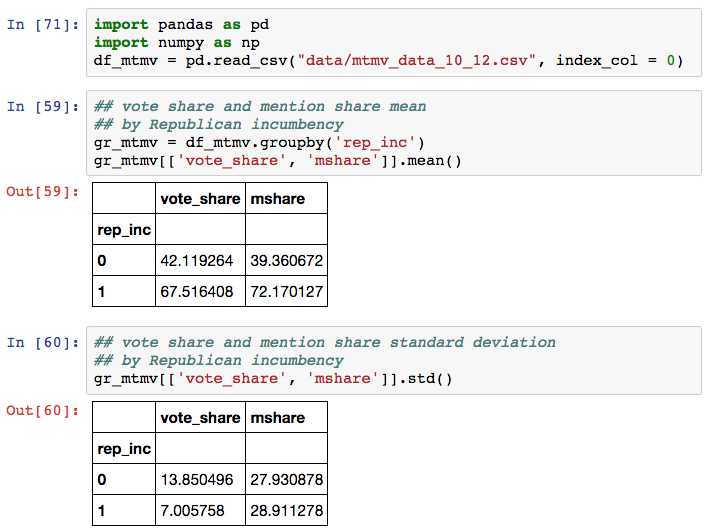
\includegraphics[width=0.9\textwidth]{img/mtmv-meansd.png}
\end{frame}

\begin{frame}{Explanation of MTMV Data: Correlation}
    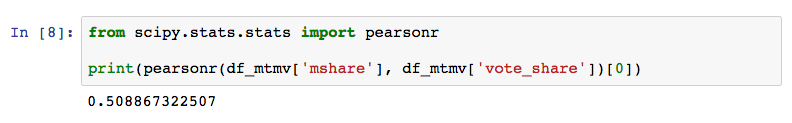
\includegraphics[width=\textwidth]{img/mtmv-correlation.png}

    \vspace*{1em}

    \textit{Pearson correlation}: measure of the linear dependence between two variables X and Y. Ranges from [-1, 1].
\end{frame}

\begin{frame}{Explanation of MTMV Data: Linear Regression}
    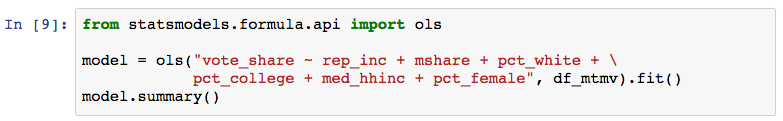
\includegraphics[width=\textwidth]{img/mtmv-ols-1.png}

    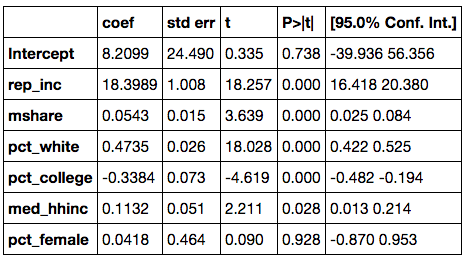
\includegraphics[width=0.7\textwidth]{img/mtmv-ols-2.png}

    \textit{Regression}: statistical technique which models the relationship between multiple variables.
\end{frame}

\begin{frame}[plain]
    \begin{center}
    \textbf{\LARGE Exercise: Build your own model!}
    \end{center}
\end{frame}

\begin{frame}{Visualisation}
    \begin{columns}
        \begin{column}{0.4\textwidth}
            Purposes of visualisation
            \begin{itemize}[<+->]
                \item Exploring data
                \item Confirming model
                \item Presenting results
            \end{itemize}
        \end{column}
        \begin{column}{0.6\textwidth}
            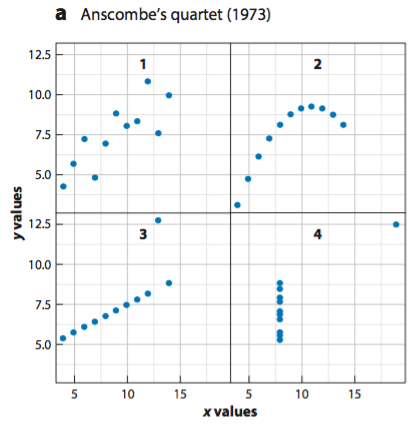
\includegraphics[width=\textwidth]{img/anscombe.png}
        \end{column}
    \end{columns}
\end{frame}

\begin{frame}{Univariate visualisations}
    \begin{columns}
        \begin{column}{0.4\textwidth}
            \begin{itemize}[<+->]
                \item Understand the variable beyond mean, median, standard deviation, etc.
                \item Should be first part of exploring data
                \item Types
                \begin{itemize}
                    \item Histogram
                    \item Density
                \end{itemize}
            \end{itemize}
        \end{column}
        \begin{column}{0.6\textwidth}
            \only<4>{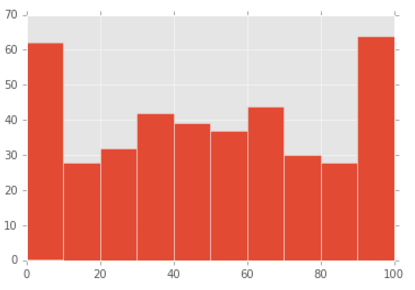
\includegraphics[width=\textwidth]{img/mshare-hist.png}}
            \only<5>{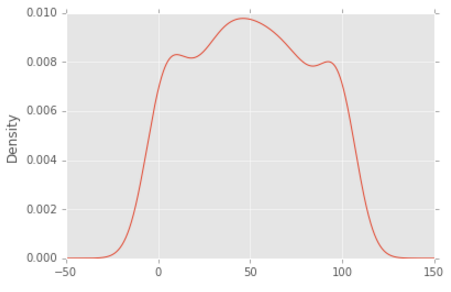
\includegraphics[width=\textwidth]{img/mshare-density.png}}
        \end{column}
    \end{columns}
\end{frame}

\begin{frame}{Univariate visualisations: Comparing variables}
    \begin{center}
        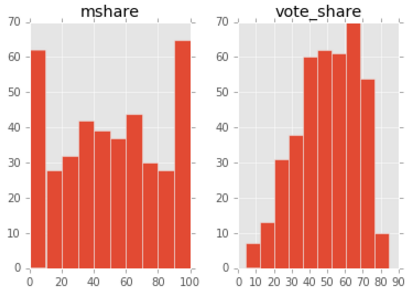
\includegraphics[width=0.8\textwidth]{img/mshare-voteshare-hist.png}
    \end{center}
\end{frame}

\begin{frame}{Bivariate and multivariate visualisations}
    \begin{columns}
        \begin{column}{0.4\textwidth}
            \begin{itemize}[<+->]
                \item Understanding variable relationships
                \item First part of model exploration
            \end{itemize}
        \end{column}
        \begin{column}{0.6\textwidth}
            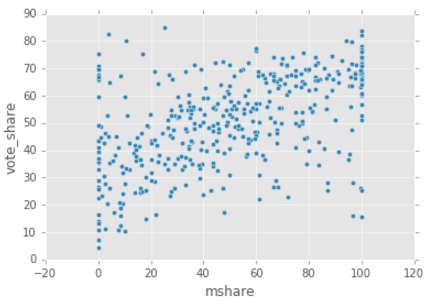
\includegraphics[width=\textwidth]{img/mshare-voteshare-scatter.png}
        \end{column}
    \end{columns}    
\end{frame}

\begin{frame}{Multivariate visualisation: Adding color}
    \begin{center}
        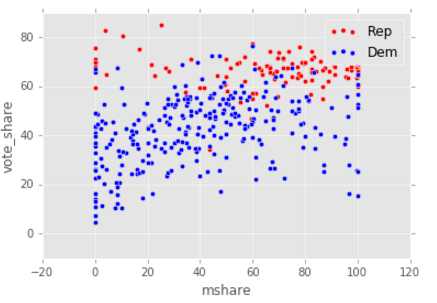
\includegraphics[width=0.8\textwidth]{img/mshare-voteshare-scatter-color.png}
    \end{center}
\end{frame}

\begin{frame}{Model confirmation}
    \begin{center}
        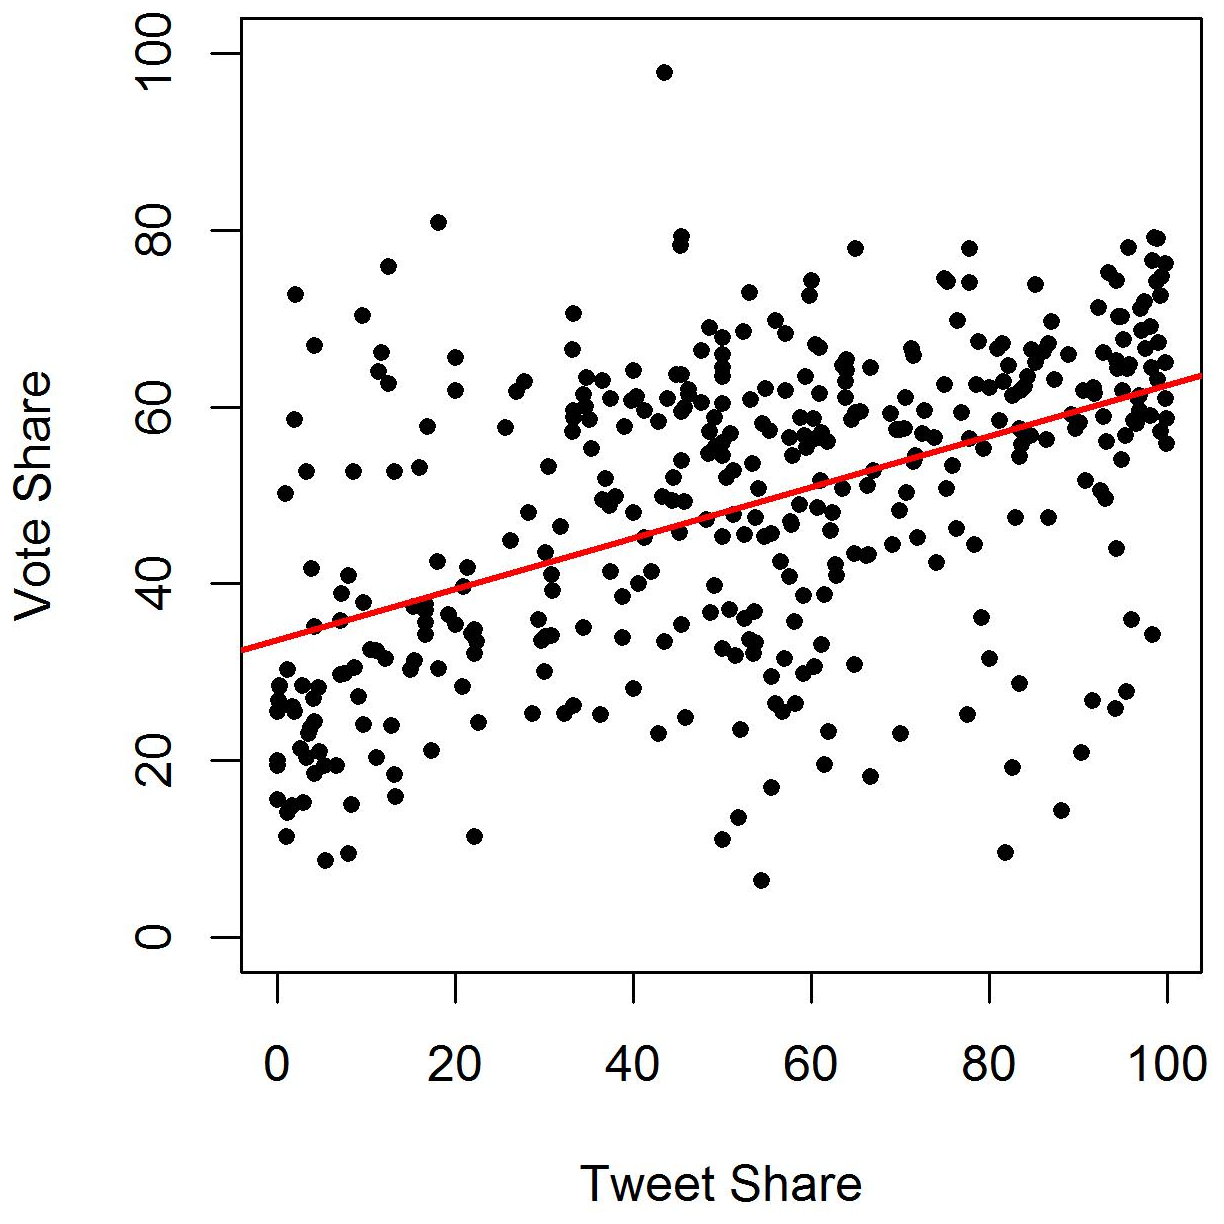
\includegraphics[width=0.6\textwidth]{img/DiGrazia-F2.png}
    \end{center}
\end{frame}

\begin{frame}[plain]
    \begin{center}
        \textbf{\LARGE guessthecorrelation.com}
    \end{center}
\end{frame}

\end{document}












